
\documentclass{article}

\usepackage[utf8]{inputenc}
\usepackage[spanish]{babel}
\usepackage{amssymb}
\usepackage{amsmath}
\usepackage{txfonts}
\usepackage{mathdots}
\usepackage{graphicx}
\usepackage{float}

%Title:
\font \authors=cmr12 at 13pt
\title{\underline{\textbf{Práctica 1: Programación Lógica pura.}}}
\author{\authors\underline{Vidal Peña, Arturo}}
\date{\today}

\begin{document}

\maketitle

\quad

\quad

\quad

\quad

\quad

\quad

\tableofcontents

 \eject 

\section{\underline{Código empleado y las explicaciones}:}
\quad
\begin{enumerate}
\item  \underline{Definición de la base de hechos de los colores de las piezas de LEGO$\mathrm{{}^{TM}}$}:\\

 Disponemos una base de hechos con los colores amarillo (am), verde (v), azul (a) y rojo (r) para hacer las comprobaciones de los colores de las piezas.\newline
 
 \begin{figure}[h]
 	\centering
 	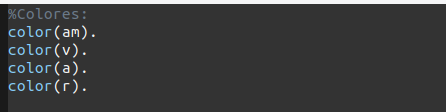
\includegraphics{images/baseColores.png}
 \end{figure}

\quad

\item  \underline{Definición de predicados auxiliares comunes a los especificados en la práctica:}\\
 

Definimos una serie de predicados auxiliares: \\

 \begin{enumerate}
\item  \underline{nat/1}: comprueba que el número pasado como argumento es un número natural. Partiendo de 0 (que definimos natural), un número X será natural si X-1 lo es.

\item  \underline{menor\_igual/2}, que será cierto si el primer argumento es menor o igual que el segundo. Se llama recursivamente con el número de Peano anterior a cada argumento hasta que el primero sea 0 y el segundo, mayor que 0.

\item  \underline{mayor\_igual/2}, su funcionamiento es igual que el anterior, sólo que comprueba si el primer argumento es mayor o igual que el segundo.

\begin{figure}[H]
	\centering
	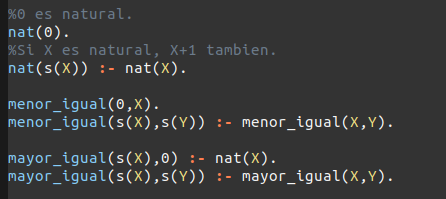
\includegraphics[width=0.75 \textwidth]{images/reglas1.png}
\end{figure}

\item  \underline{suma/3}, que será cierto cuando el tercer argumento sea la suma aritmética de los dos primeros.

\item  \underline{resta/3}, que será cierto cuando el tercer argumento sea la resta aritmética de los dos primeros.
\item  \underline{iguales/2}, será cierto cuando ambos argumentos pasados como números de Peano tengan el mismo valor. Se llama recursivamente comprobando que lleguen a 0 al mismo tiempo.

\item  \underline{par/1}: será cierto si, restando 2 al número pasado por argumento recursivamente, se llega a 0.

\item  \underline{impar/1}: igual que el anterior, sólo que comprobando que llega a 1.

\begin{figure}[H]
	\centering
	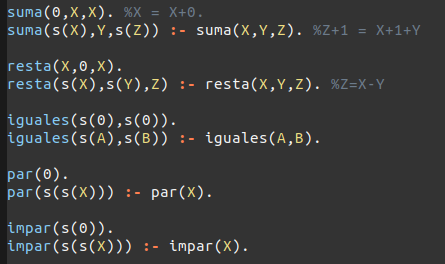
\includegraphics[width=0.75 \textwidth]{images/reglas2.png}
\end{figure}

\item  \underline{esPieza/4}: comprueba si los argumentos \textit{Altura}, \textit{Anchura} y \textit{Profundidad} pasados como números de Peano son naturales, y si \textit{Color} está en la base de hechos.

\item  \underline{p/3}: siendo pasada una lista como primer argumento, será cierto si el segundo argumento es la cabeza y el tercero, la cola de la lista.

\item  \underline{member/2}: comprueba si el primer argumento se encuentra en la lista que se pasa en el segundo argumento.

\begin{figure}[H]
	\centering
	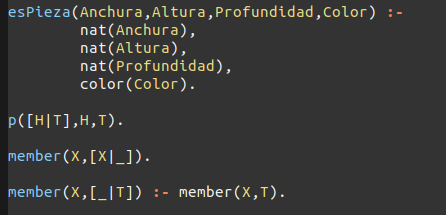
\includegraphics[width=0.75 \textwidth]{images/reglas3.png}
\end{figure}


\end{enumerate}


\item  \underline{Definición del predicado esTorre/1}:\\

 El caso base se afirma si la torre se compone de una única pieza, llamando a esPieza/1.

 En el caso de tener más de una pieza, comprueba recursivamente que las piezas de la torre son válidas con esPieza/1 y que la pieza en cabeza es más pequeña en \textit{Anchura} y \textit{Profundidad} que la siguiente en la torre, llegando al caso base con la última pieza.

\begin{figure}[H]
	\centering
	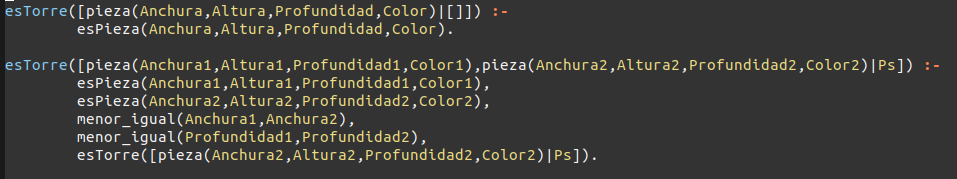
\includegraphics[width=0.75 \textwidth]{images/esTorre.png}
\end{figure}



\item  \underline{Definición del predicado alturaTorre/2}:\\

 El caso base se afirma si la torre de una única pieza es válida (esTorre/1), si el segundo parámetro en natural, y si este segundo parámetro vale 0 al ser restado por la altura de la pieza que conforma la torre.

 En el caso de haber más de una pieza, comprueba que la lista es una torre válida, comprueba que el segundo parámetro es un natural, y llama al predicado auxiliar exclusivo de alturaTorre/2, pasando los mismos argumentos. Este predicado sacarAltura/2 va restando recursivamente al segundo parámetro las alturas de las piezas que conforman la torre, llegando al caso base con la última pieza.

\begin{figure}[H]
	\centering
	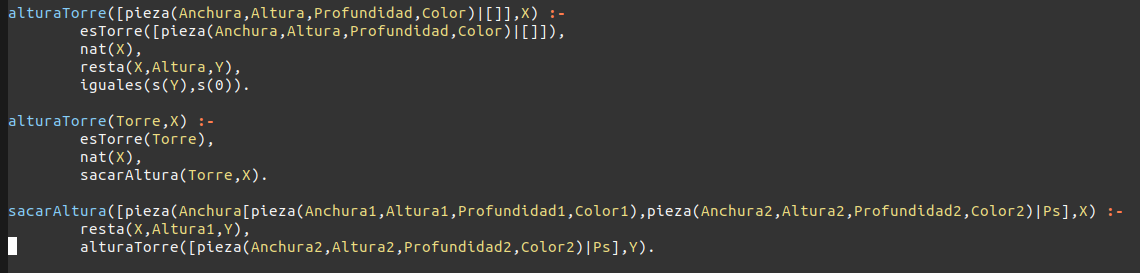
\includegraphics[width=0.75 \textwidth]{images/alturaTorre.png}
\end{figure}

\newpage

\item  \underline{Definición del predicado coloresTorre/2}:\\

 El caso base se afirma si la torre de una única pieza es válida (esTorre/1), y si el color de la pieza pertenece a la lista de colores pasada en el segundo parámetro.

 En el caso de haber más de una pieza, comprueba si la lista es una torre válida, si el segundo parámetro es un número natural, y luego llama al predicado auxiliar exclusivo de coloresTorre/2, pasando los mismos argumentos. Este predicado sacarColores/2 comprueba recursivamente que los colores de las piezas de la torre pertenecen a la lista de colores del segundo parámetro, llegando al caso base con la última pieza.

\begin{figure}[H]
	\centering
	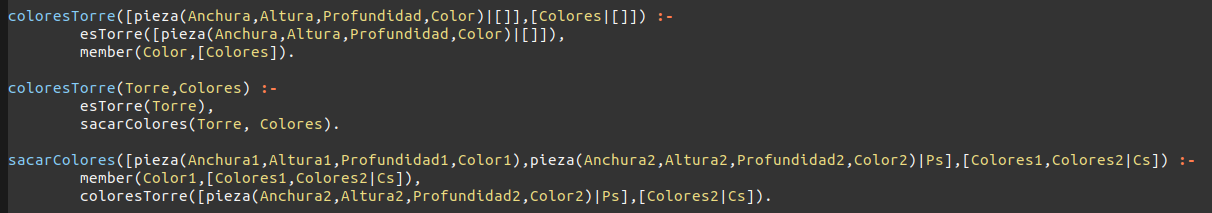
\includegraphics[width=0.75 \textwidth]{images/coloresTorre.png}
\end{figure}


\item  \underline{Definición del predicado coloresIncluidos/2, junto a sus auxiliares}:\\

 Primero comprueba si ambas torres pasadas como parámetros son válidas, y luego llama al predicado auxiliar exclusivo de coloresIncluidos, pasando la primera torre en el primer parámetro y la segunda, en el segundo y tercero.

 Este predicado (comprobarColores/3), compara recursivamente el primer color de Torre1 con los colores de Torre2. Cuando acaba, copia la Torre2 y vuelve a empezar con el siguiente color de Torre1.

\begin{figure}[H]
	\centering
	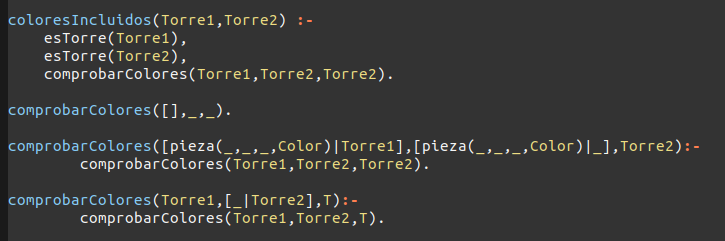
\includegraphics[width=0.75 \textwidth]{images/coloresIncluidos.png}
\end{figure}


 
\item  \underline{Definición del predicado esEdificioPar/1, junto a sus auxiliares}:\\

 El caso base de esEdificioPar/1 es si la construcción sólo tiene una línea, en cuyo caso será cierto si esa línea es par, llamando al predicado lineaPar/1. En el caso de haber más de una línea, comprobará con lineaPar/1 si todas las líneas de la construcción son pares.

 Este predicado auxiliar llama a longitudLinea/2, pasando la línea y una variable en la que unificar la longitud de esta. Este predicado llama a su vez a longitudSinBlanco/3, pasando la línea, inicializando N1 a 0 y la variable a unificar en N2. 

 En longitudSinBlanco/1, si la cabeza de Linea es un blanco, se llama recursivamente con la cola de Linea como primer argumento. En otro caso, comprueba que la cabeza es un color válido, y se llama recursivamente con la cola como primer argumento, y el siguiente a N1 como segundo, siendo N2 siempre el tercero. Al acabar, cuando la línea está vacía, iguala N2 a N1.

  Al unificar N2 con el segundo argumento de longitudLinea/2, comprueba que sea un número par con par/1. Si es cierto, la línea es par.

\begin{figure}[H]
	\centering
	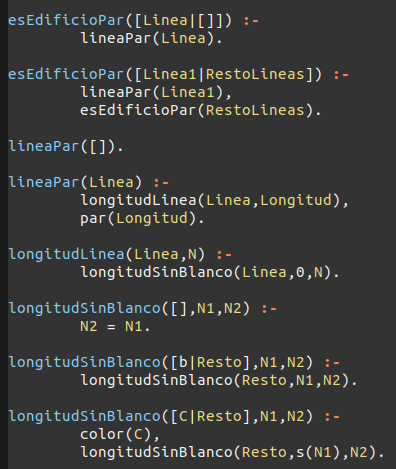
\includegraphics[width=0.75 \textwidth]{images/esEdificioPar.png}
\end{figure}


 
%\item  \underline{Definición del predicado esEdificioPirámide/1 y sus auxiliares}:

\end{enumerate}

\newpage

\section{\underline{Pruebas realizadas}:}

Todas las pruebas a continuación han dado los valores esperados.

\begin{enumerate}
	\item \underline{nat/1}:
	\begin{itemize}
	\item nat(0),            
	\item nat(s(0)),
	\item nat(s(s(s(s(0))))),
	\item nat(t)
	\end{itemize}
	
	\item \underline{menor\_igual/2}:
	\begin{itemize}
	\item menor\_igual(s(0),s(0)),             
	\item menor\_igual(s(s(0)),s(s(0))),
	\item menor\_igual(s(0),s(s(0)))
	\end{itemize}

\item \underline{resta/2}:
\begin{itemize}
	\item resta(s(0),0,s(0)),            
	\item resta(s(0),s(0),0),             
	\item resta(s(s(s(s(0)))),s(s(s(s(0)))),0)
\end{itemize}

\item \underline{par/1}:
\begin{itemize}
	\item par(0)             
	\item par(s(s(0))),             
	\item par(s(s(s(s(0)))))
\end{itemize}

\item \underline{iguales/2}:
\begin{itemize}
	\item iguales(s(0),s(0)),             
	\item iguales(s(0),s(0)),             
	\item iguales(s(s(s(s(0)))),s(s(s(s(0))))),
\end{itemize}

\item \underline{color/1}:
\begin{itemize}
	\item color(r),             
	\item color(v),             
	\item color(am),
	\item color(a),
	\item color(b)
\end{itemize}

\item \underline{esTorre/1}:
\begin{itemize}
	\item esTorre([pieza(s(0),s(s(0)),s(0),r)]),             
	\item esTorre([pieza(s(0),s(s(0)),s(0),r),pieza(s(0),s(0),s(0),a)]),             
	\item esTorre([pieza(s(s(s(0))),s(s(s(0))),s(s(s(0))),am),pieza(s(s(s(0))),s(s(s(0))),s(s(s(0))),v)])
\end{itemize}

\item \underline{alturaTorre/2}:
\begin{itemize}
	\item alturaTorre([pieza(s(0),s(0),s(0),r)],s(0)),             
	\item alturaTorre([pieza(s(0),s(0),s(0),r),pieza(s(s(0)),s(s(0)),s(0),a)],s(s(s(0)))),   
	\item alturaTorre([pieza(s(0),s(0),s(0),r),pieza(s(0),s(0),s(0),r),pieza(s(0),s(s(0)),s(0),r)],s(s(s(s(0)))))
\end{itemize}

\item \underline{coloresTorre/2}:
\begin{itemize}
	\item coloresTorre([pieza(s(0),s(0),s(0),r)],[r]),             
	\item coloresTorre([pieza(s(0),s(0),s(0),r),pieza(s(0),s(s(0)),s(0),a)],[r,a]),             
	\item coloresTorre([pieza(s(0),s(s(0)),s(0),am),pieza(s(0),s(0),s(0),r),pieza(s(0),s(s(0)),s(0),a)],[am,r,a])
\end{itemize}

\item \underline{coloresIncluidos/2}:
\begin{itemize}
	\item coloresIncluidos([pieza(s(0),s(0),s(0),r)],[pieza(s(0),s(0),s(0),r)]),             
	\item coloresIncluidos([pieza(s(0),s(0),s(0),a),pieza(s(0),s(0),s(0),a)],[pieza(s(s(0)),s(0),s(s(0)),a)]),             
	\item coloresIncluidos([pieza(s(0),s(0),s(0),r),pieza(s(0),s(0),s(0),v),pieza(s(0),s(0),s(0),a)])
\end{itemize}

\item \underline{esEdificioPar/2}:
\begin{itemize}
	\item esEdificioPar([[a,a],[v,v],[a,a],[v,v]]),             
	\item esEdificioPar([[a,a,r,v,am,r],[v,r,v,v,am,r],[v,r,v,r,a,r],[v,r,a,r,v,r],[v,r,a,r,v,am]]),             
	\item esEdificioPar([[a,a,am,r],[v,v,am,r],[v,r,a,r],[v,r,a,r],[v,r,a,am]])
\end{itemize}

%\item \underline{esEdificioPiramide/2}:
%\begin{itemize}
%	\item esEdificioPiramide([[b,b,b,r,b,b,b],[b,am,r,b,b,b,b]]),             
%	\item esEdificioPiramide([[b,am,b],[b,am,r]]),             
%	\item esEdificioPiramide([[b,b,v,b,b],[b,a,r,a,b]])
%\end{itemize}
\end{enumerate}

\end{document}

